% LaTex file for Stephen Balakirsky's Robotics and 
% Computer Integrated Manufacturing 2014 submission
%
\documentclass[review]{elsarticle}

\usepackage{lineno,hyperref}

%
% my additional packages
\usepackage{graphicx}
\usepackage{multirow,array}
\usepackage{rotating} % for sideways
\usepackage{amsmath}
\usepackage{amsthm}
%\usepackage{algorithm2e}
\usepackage[linesnumbered, boxed, figure]{algorithm2e}
%
% zeid's definitions
\newcommand{\class}[1] {\textit{#1}}
\newcommand{\const}[1] {$\mathit{#1}$}
\newcommand{\objvar}[1] {$\mathsf{#1}$}
\newcommand{\stvar}[1] {\textsf{#1}}
%
%
%
\modulolinenumbers[5]

\journal{Journal of Robotics-and-Computer-Integrated-Manufacturing}

%%%%%%%%%%%%%%%%%%%%%%%
%% Elsevier bibliography styles
%%%%%%%%%%%%%%%%%%%%%%%
%% To change the style, put a % in front of the second line of the current style and
%% remove the % from the second line of the style you would like to use.
%%%%%%%%%%%%%%%%%%%%%%%

%% Numbered
%\bibliographystyle{model1-num-names}

%% Numbered without titles
%\bibliographystyle{model1a-num-names}

%% Harvard
%\bibliographystyle{model2-names.bst}\biboptions{authoryear}

%% Vancouver numbered
%\usepackage{numcompress}\bibliographystyle{model3-num-names}

%% Vancouver name/year
%\usepackage{numcompress}\bibliographystyle{model4-names}\biboptions{authoryear}

%% APA style
%\bibliographystyle{model5-names}\biboptions{authoryear}

%% AMA style
%\usepackage{numcompress}\bibliographystyle{model6-num-names}

%% `Elsevier LaTeX' style
\bibliographystyle{elsarticle-num}
%%%%%%%%%%%%%%%%%%%%%%%

\begin{document}

\begin{frontmatter}

\title{Ontology Based Action Planning and Verification for Agile Manufacturing}

%% Group authors per affiliation:
\author{Stephen Balakirsky}
\address{Georgia Tech Research Institute, Atlanta, GA 30332, USA}
\cortext[mycorrespondingauthor]{Corresponding author}
\ead{stephen.balakirsky@gtri.gatech.edu}

\begin{abstract}
Many of today's robotic work cells are unable to adapt to even small changes in tasking without significant reprogramming. 
This results in downtime for production
lines anytime a change to a product or procedure must be made. This article examines a novel 
knowledge-driven system that 
provides added agility by removing the programming burden for new activities from the robot 
and placing it in the knowledge representation. The system is able to automatically 
recognize and adapt to changes in its work-flow and dynamically change assignment details. 
The system also provides for 
action verification and
late binding of action parameters, 
thus providing flexibility by allowing plans 
to adapt to production errors and changing environmental conditions. The key feature of this system is its knowledge base that 
contains the necessary 
relationships and representations to allow for
adaptation. This article presents the ontology that stores this knowledge as well as the 
overall system architecture. 
The manufacturing domain of kit construction is examined as a sample test environment. 
\end{abstract}

\begin{keyword}
\texttt{knowledge driven system, adaptive planning, manufacturing, ontology, robotics, Planning Domain Definition Language}
\end{keyword}

\end{frontmatter}

\linenumbers

%
%\usepackage{makeidx}  % allows for indexgeneration
%
%
%
\section{Introduction}
A failure is any change, design, or manufacturing error that renders a component, assembly, or system incapable of performing its intended function \cite{Collins93}. In kitting, as described in Section \ref{sect:kitting}, failures can occur for multiple reasons that include equipment not being set up properly, tools and/or fixtures not being properly prepared, and improper equipment maintenance. Part/component availability failures can be triggered by inaccurate information on the location of the part, part damage, incorrect part types, or part shortage due to delays in internal logistics. In order to prevent or minimize failures, a disciplined approach needs to be implemented to identify the different ways a process design can fail before impacting productivity.

Even though today's state-of-the-art industrial robots are capable of sub-millimeter accuracy \cite{RobotAccuracy}, they often lack the sensing
necessary to detect failures and the programming required to cope with and correct the failure. This is due to the fact that they are often programmed
by an operator using crude positional controls from a teach pendant. These teach pendant programs are highly repeatable, which provides 
utility for large-batch, error-free operation. However, the cyclic program that repeats identical operations does not lend itself well to adaptation for 
failure mitigation. In fact, producing a program to correct a perceived failure would require that the cell be taken off-line
for additional human-led teach pendant programming. In addition, 
most cells lack the ability to sense that a failure occurred and  lack programming (that would have had to be teach pendant entered) to cope
with failure conditions, thus making it impossible for the cell to recover from failures.
This leads to faulty products being sent down the line, and/or downtime for the cell as failures are detected and corrected.

For small batch processors or other customers who must frequently change their line configuration or desire to perform complex operations
with their robots, this frequent downtime and lack of failure correction/detection may be unacceptable. The robotic systems of tomorrow need to be capable, flexible, and agile.  
These systems need to perform their duties at least  as well as human counterparts, be quickly re-tasked to other operations, cope with a wide 
variety of unexpected environmental and operational changes, and be able to detect and correct errors in operation. 
To be successful, these systems need to combine domain expertise, knowledge of their own skills and limitations, and both semantic and geometric 
environmental information.

The IEEE Robotics and Automation Society's Ontologies for Robotics and Automation Working Group has taken the first steps in creating the 
infrastructure necessary for such a system, while the Industrial Subgroup has applied this infrastructure to create a sample kit building
system.  This work is presented in Balakirsky et al. \cite{balakirsky2013} which describes the construction of a robotic kit building
system that is able to cope with environmental and task changes without operator intervention. This article extends that work to utilize
the same infrastructure to allow for the detection and correction of action failures in the system.

The organization of the remainder of this paper is as follows. Section \ref{sect:kitting} describes the domain of kit building. Section \ref{sect:overview} presents
an overview of the software system architecture as well as details of the ontology and world model for the robot cell. Section \ref{sect:operation} discusses the detailed operation of cell, and Section \ref{sect:failure} discusses how failures are handled by the ontology. Finally, Section \ref{sect:future} presents
conclusions and future work.
%
%
\section{Kitting}
\label{sect:kitting}
Today's advanced manufacturing plants utilize mixed-model assembly where multiple product variants are built on the same line.  
According to Jim Tetreault, Ford’s vice president of North America Manufacturing, 
new Ford assembly facilities are able to build a full spectrum of vehicles on the same assembly line \cite{James2011}. One of the technologies that makes this possible
is the use of assembly kits.  Bozer and McGinnis \cite{Bozer1992} describe a kit as ``a specific
collection of components and/or subassemblies that together (i.e., in the same container) support one or more assembly
operations for a given product or shop order''. These  kits provide a synchronous material flow, where parts and components move to 
assembly stations in a just-in-time manner. The kits provide workers with the parts and tools that they need (which may vary from 
vehicle model to vehicle model) in the sequence that they need them. The use of kitting also allows a single delivery system to feed
multiple assembly stations thus saving manufacturing or assembly space \cite{Medbo2003} and provides an additional inspection opportunity 
that allows for the detection of part defects before they impact assembly operations. The individual operations of the station 
that builds the kits may be viewed as a specialization of the general
bin-picking problem \cite{Schyja2012} where parts are picked from one or more part bins or trays and placed into specific slots in a kit tray.

For our sample implementation, we assume that the robot cell is building one of several possible kit configurations. At execution time, the
cell has a set kit to build, but does not know the precise location of the kit tray, the part trays, or the location of individual parts in the part tray.
When a human builds a kit, they are able to inspect each part before adding it to the kit tray. This provides an additional level of quality control and
is an aspect that is desirable to have in our robotic system. During kit construction,
a robot performs a series of pick-and-place operations
in order to construct the kit. These operations include:
\begin{enumerate}
\item Pick up an empty kit and place it on the work table.
\item Pick up multiple component parts, inspect them, and place them in the kit.
\item Pick up the completed kit and place it in the full kit storage area.
\end{enumerate}
Each of these steps may be a compound action that includes
other actions such as end-of-arm tool changes, path planning,
and obstacle avoidance. The items that are being placed in the kit may be of varying size and shape and have various grasping and inspection
requirements.
%
\begin{figure}[htb!]
\begin{center}
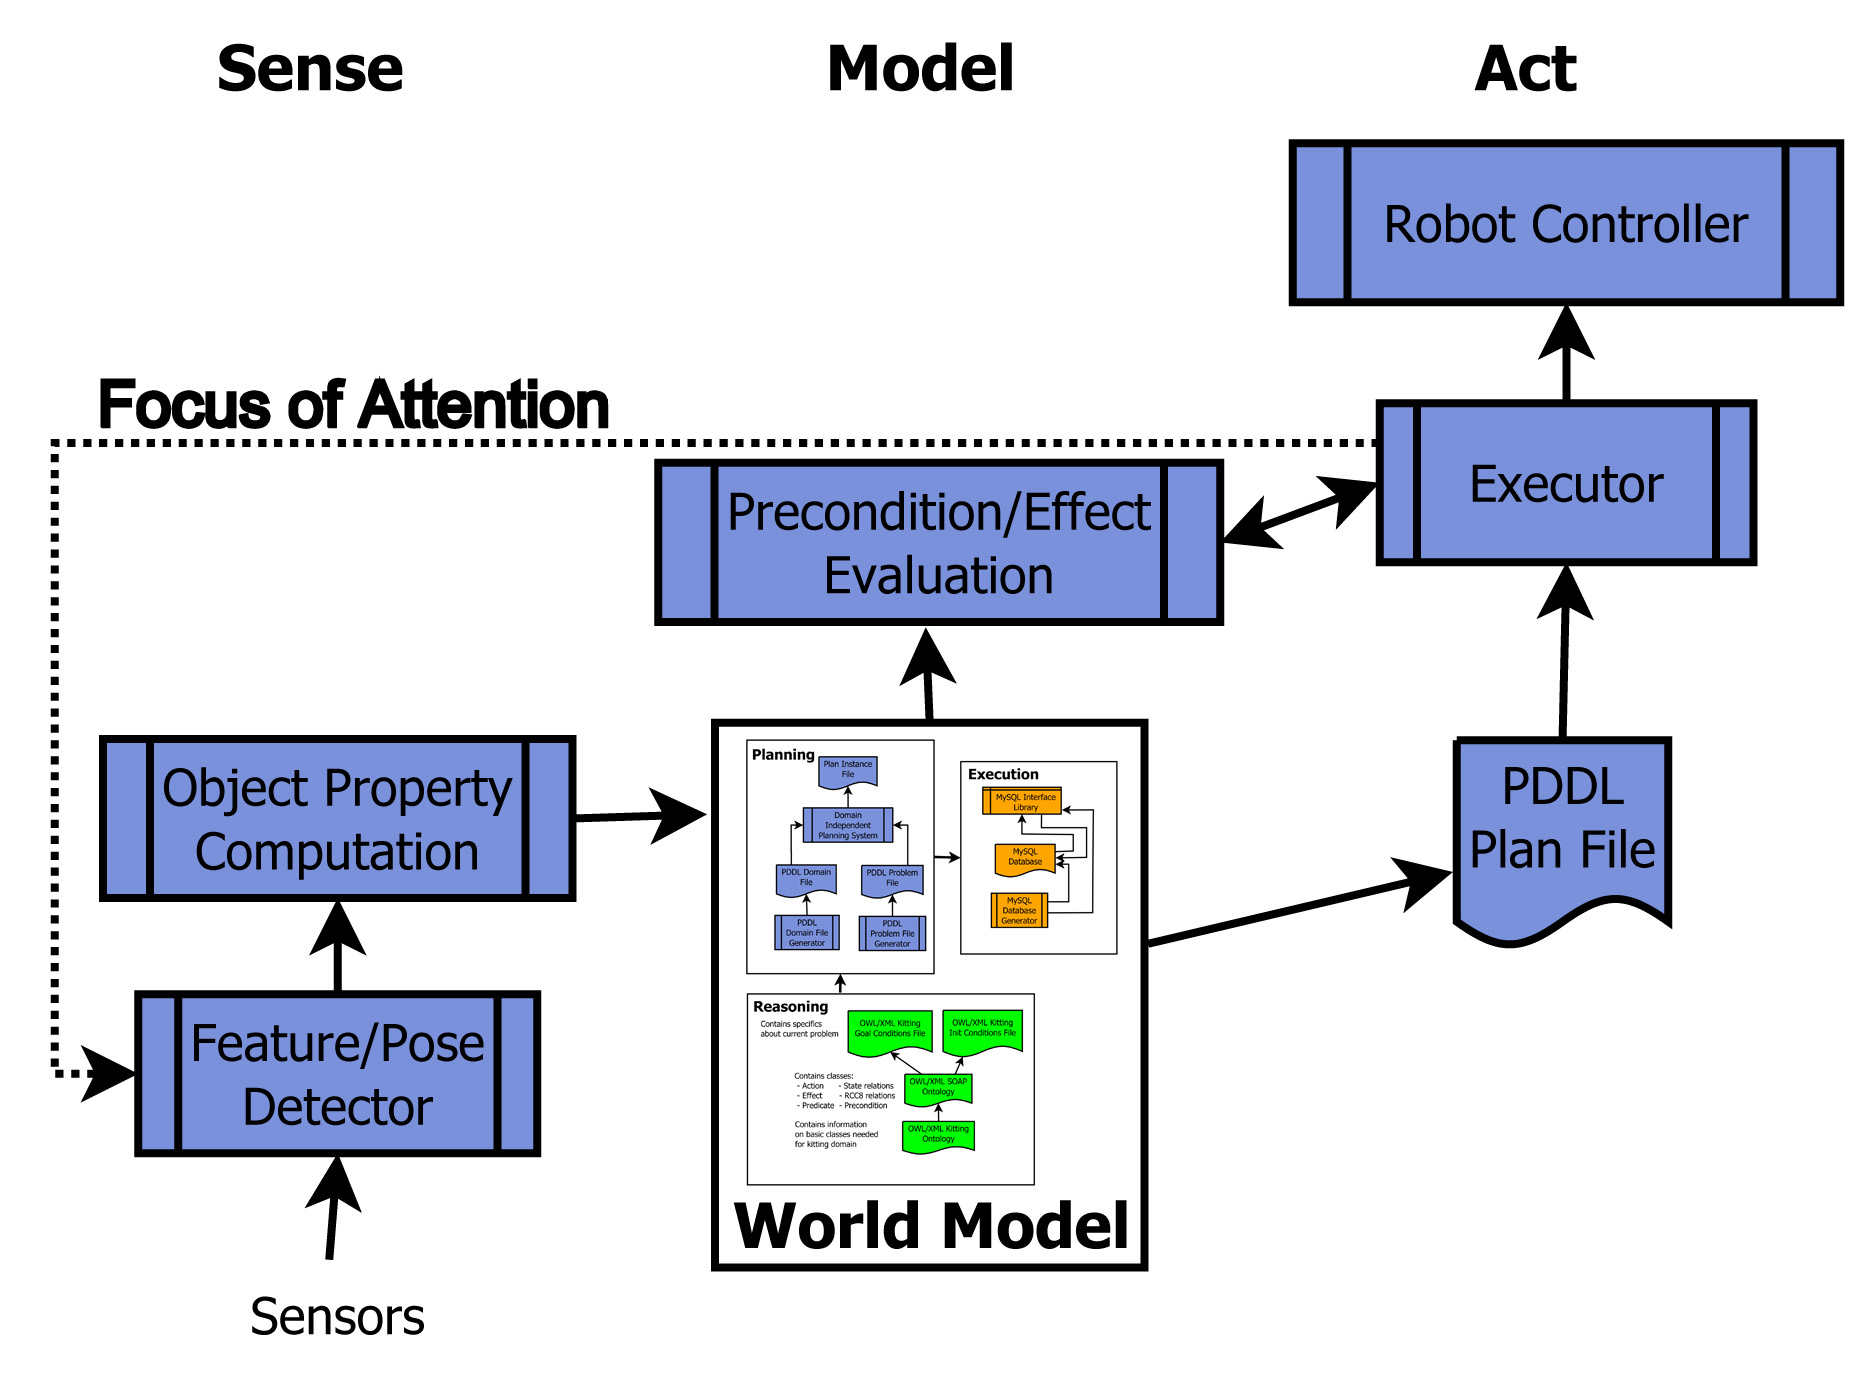
\includegraphics[width=8.5cm]{images/RITAExecution.jpg}
\caption{Major components that make up the Sense--Model--Act paradigm of the kitting station.}
\label{fig:SenseModelAct}
\end{center}
\end{figure}
%
\section{PDDL}
\label{sect:PDDL}
The objective behind domain independent planning is to formulate a
planner that is able to construct plans across a wide variety of planning domains with 
no change to the planning algorithms. The typical problem presented to such a planner
consists of:
%
\begin{itemize}
\item A set of objects,
\item A set of predicate expressions that define properties of
objects and relations between objects,
\item A set of actions that are able to manipulate the predicate
expressions,
\item A set of predicate expressions that constitute a partial
world state and make up the initial conditions,
\item A set of problem goals, which are predicate expressions that are required to be 
true at the end of a plan.
\end{itemize}
%
If an {\it action} is defined as a fully-instantiated operator, then the job of the planner is to formulate a sequential list of valid actions, referred to as a {\it valid plan}, which will bring the system from the state represented by the initial conditions to a state that satisfies the problem goals (all of the problem goals are simultaneously true).
%
\begin{figure}[htb!]
\begin{center}
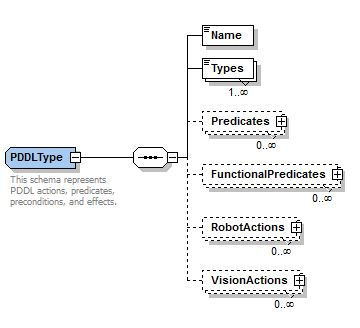
\includegraphics[width=8.5cm]{images/PDDLType.jpg}
\caption{Description of the PDDLType class that is designed as
an augmented PDDL description language. It contains all of the
information necessary for interacting with the robot cell's
robot controller and vision system.}
\label{fig:pddlType}
\end{center}
\end{figure}
%

PDDL is designed as a standard language and structure for 
representing a valid plan along with all of the elements of
domain independent planning systems. Figure \ref{fig:pddlType}
depicts a schema view of our augmented PDDL representation.
As in a standard PDDL representation, a set of object {\it types} 
is represented along with \textit{predicate} expressions and 
{\it actions}. The schema has been augmented with the
representation of \textit{functionalPredicates} and
the distinction between \textit{RobotActions} and
\textit{VisionActions}.

In PDDL, {\it types} must be declared before their use as
parameters to predicate expressions. For our PDDL extension,
the additional requirement has been added that all types must
be defined in the system's ontology and must be derived from the base
\textit{SolidObject} or \textit{SystemConstant}
classes. This assures that basic properties of
objects being used as parameters are known to the system.
The \textit{SolidObject} provides the basis for all physical
objects in the world while the \textit{SystemConstant}
represents a named system memory location that may be used as intermediate 
storage of values between commands. It is often used by \textit{VisionActions}
to store values required by a future \textit{RobotAction}.

\textit{Predicates} are binary expressions that contain one or 
two objects
of defined \textit{types} as arguments and provide a partial 
definition of the world's state. Predicates may be used for 
\textit{preconditions} (predicates that must be true for an
action to be executed) as well as \textit{effects} (predicates
that are expected to become true as the result of an action).
An additional class of predicates known as \textit{FunctionalPredicates}
has been added to this representation. These predicates allow for
mathematical operations to be performed between parameters. For example,
the predicate \textit{equalTo(obj1, value)} will evaluate the
equivalence between \textit{obj1} and \textit{value} while the predicate
\textit{set-value(systemVariable, setValue, valueType)} will set the value of the variable 
\textit{systemVariable} to \textit{setValue}. The \textit{set-value} predicate
will evaluate to \textit{true} if the memory location to be set exists and the value
to be set is of the correct type for that memory location.

\textit{Actions} represent compound tasks that the robot cell must accomplish.
Our robot cell consists of a robotic arm and a vision system. Therefore, our
actions have been segregated into \textit{RobotActions} that pertain to the robot system
and \textit{VisionActions} that pertain to the vision system.
More information on the implementation of these types in the ontology may be found in Section \ref{sect:knowledge}. 

\section{System Operation}
\label{sect:operation}
In order to construct a kit, the kitting system steps through each action in
the precomputed PDDL plan. Failures are searched for both before and after execution of 
each action. The overall process, known as {\sc BuildKit} is shown in Figure
\ref{fig:buildkit}. 

This process begins by retrieving a planning instance that has been 
precomputed to solve the construction of the requested kit (Line 1 of 
Figure \ref{fig:buildkit}). This is a high-level PDDL
plan that is not grounded to actual part instances or locations. It contains information
on the named storage location for classes of parts (individual SKU numbers), 
the quantity of each SKU that is required by the kit, and a build order (a sequence
of SKUs to be added to the kit). Additional information on the appropriate
end-of-arm tooling required to grip each part is also included.

This planning instance is decomposed into individual actions that must
be successfully carried out to complete the construction of the kit (the
{\it for} loop beginning at Line 2 of Figure \ref{fig:buildkit}). At this point,
preconditions of the action are examined to assure that the action to be attempted
is valid. If any of the action's preconditions are not able to be validated,
a failure is reported; otherwise, the action is approved for execution.
%
\begin{algorithm}[h!]
 \KwData{ $PredicateIn$ }
 \KwResult{true or false}
 	determine predicted pose $PoseR$ of $PredicateIn.ReferenceParameter$
 	and $PoseT$ of $PredicateIn.TargetParameter$ \;
 	send $PredicateIn$, pose $PoseR$, and $PoseT$ as focus of attention command to $SensorProcessing$\;
   	\uIf{$Eval(PredicateIn) == true$}{
 		return true\;
 	}
 	\Else{
 		return false \;
 	}
\caption{{\sc PredicateEvaluation} -- Returns the truth value of the predicate expression.}
\label{fig:predicateEval}
\end{algorithm}
%
\subsection{Precondition Validation}
\label{sect:preconditionValid}
Each precondition is a predicate expression that must be validated prior to
action execution.
The procedure for validating predicates is shown in Figure \ref{fig:predicateEval}. In Line 1 of this algorithm, the world
model is queried for the pose and class of each relevant 
parameter of the predicate. The information returned is the 
latest knowledge that has been recorded by the sensor processing
system and is not guaranteed to be up-to-date. This predicted
knowledge is sent as a focus of attention indicator to the sensor
processing system, and the sensor processing system is instructed to
update the predictions in the world model with current observations
and to compute the supporting relationships necessary for predicate
evaluation.
%
\begin{algorithm}[h!]
 \KwData{ $PredicateIn, PoseR, PoseT$ }
 	determine actual pose $APoseR$ of $PredicateIn.ReferenceParameter$\;
 	determine actual pose $APoseT$ of $PredicateIn.TargetParameter$\;
 	determine RCC8 relations between $APoseR$ and $APoseT$\;
 	determine Intermediate State Relations based on RCC8 relations\;
 	determine truth value of $PredicateIn$ and write to MySQL database\;
\caption{{\sc SensorProcessing} -- Updates the MySQL database in the Execution world model
to contain the latest evaluation of predicates related to $PredicateIn$.}
\label{fig:sensorProcess}
\end{algorithm}
%
Figure \ref{fig:sensorProcess} depicts the algorithm that is followed by
sensor processing in the computation of predicate values. As may be seen from this
figure, the computation of predicates is a three step process that involves
the computation of increasingly complex forms of spatial relations. These
relationships; Region Connection Calculus (RCC8) relations, intermediate state relations, and predicate relations, are each represented as a separate class in
the ontology.
%
\subsubsection{RCC8 Relation --}
RCC8 \cite{Wolter2000} is an approach for representing the relationship between two regions in Euclidean or topological space. The class \class{RCC8\_Relation} 
is based on the definition of RCC8 and consists of eight possible relations that include Tangential Proper Part (TPP), Non-Tangential Proper Part(NTPP), Disconnected (DC), Tangential Proper Part Inverse (TPPi), Non-Tangential Proper Part Inverse (NTPPi), Externally Connected (EC), Equal (EQ), and Partially Overlapping (PO). In order to represent these relations in all three dimensions for the kitting domain, RCC8 has been extended to a three-dimensional space by applying it along all three planes (x-y, x-z, y-z) and by including cardinal direction relations ``+'' and ``-''. In the ontology, RCC8 relations and cardinal direction relations are represented as subclasses of the class \class{RCC8\_Relation}. 
%
\subsubsection{Intermediate State Relation --}
These relations can be inferred from the combination of RCC8 and cardinal direction relations. For  instance, the intermediate state relation \textbf{In-Contact-With} is used to describe that object \textit{obj1} is in contact with object \textit{obj2}. This is true if \textit{obj1} is externally connected to \textit{obj2} in the x-direction, the y-direction, or the z-direction,  and is represented with the following combination of RCC8 relations:
\begin{gather}
\textbf{In-Contact-With}(\textit{obj1}, \textit{obj2}) \rightarrow   \notag\\
\texttt{x-EC}(\textit{obj1}, \textit{obj2}) \vee \texttt{y-EC}(\textit{obj1}, \textit{obj2}) \vee \texttt{z-EC}(\textit{obj1},\textit{obj2}) \notag
\end{gather}
In the ontology, intermediate state relations are represented with the OWL built-in property \texttt{owl:equivalentClass} that links the description of the class \class{Intermediate\_State\_Relation} to a logical expression based on RCC8 relations from the class \class{RCC8\_Relation}.
\subsubsection{Predicate Relation --} The truth-value of predicates can be determined through the logical combination of intermediate state relations. The predicate \class{endeffector-location-endeffectorholder}(\textit{endeffector}, \textit{endeffectorholder}) is true if and only if the location of the end effector \textit{endeffector} is in the end effector holder \textit{endeffectorholder} and is not attached to a robot. This predicate can be described using the following combination of intermediate state relations:
\begin{gather}
\textsf{endeffector-location-endeffectorholder}(\textit{endeffector},\textit{endeffectorholder}) \rightarrow   \notag\\
\textbf{In-Contact-With}(\textit{endeffector}, \textit{enfectorholder}) \wedge \notag\\
\neg\textbf{In-Contact-With}(\textit{endeffector}, \textit{robot}) \notag
\end{gather}
As with state relations, the truth-value of predicates is captured in the ontology using the \texttt{owl:equivalentClass} property that links the description of the class \class{Predicate} to the logical combination of intermediate state relations from the class \class{Intermediate\_State\_Relation}.
\subsubsection{Truth Value Determination --}
As seen in Section \ref{sect:Ontology}, a predicate can have a maximum of two parameters. In the case where a predicate has two parameters, the parameters are passed to the intermediate state relations defined for the predicate, and are in turn passed to the RCC8 relations were the truth-value of these relations are computed. In the case the predicate has only one parameter, the truth-value of intermediate state relations, and by inference, the truth-value of RCC8 relations will be tested with this parameter and with every object in the environment in lieu of the second parameter. Our kitting domain consists of only one predicate that has no parameters. This predicate is used as a flag in order to force some actions to come before others during the formulation of the plan. Predicates of this nature are not treated in the concept of ``Spatial Relation''.

These truth values may be retrieved from the ontology for use in Line 3 of Figure
\ref{fig:predicateEval} which will then propagate back up to {\sc BuildKit}. If
the predicates are successfully evaluated, the action will be cleared for 
execution and a set of CRCL Commands will be 
generated.
%
\begin{figure}[htb!]
\begin{center}
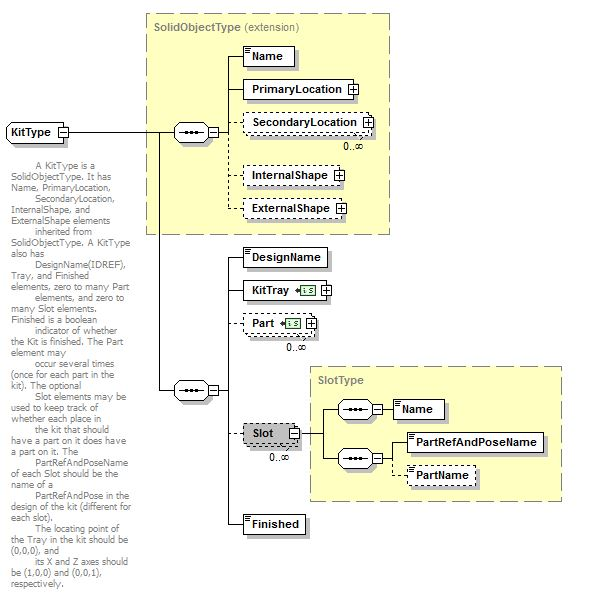
\includegraphics[width=12cm]{images/Kit.jpg}
\caption{Description of the KitType class that is designed to bring together
a container (the KitTray), a design for the kit creation, and specific parts
that populate the kit.}
\label{fig:kit}
\end{center}
\end{figure}
%
\subsection{Canonical Robot Control Language Generation}
Up to this point, the PDDL actions are not fully grounded to specific instances
that exist in the world. For example, the action \texttt{put-part} is designed
to place the part that is currently being held by the robot into a kit that
is specified as one of the action's input parameters. However, the precise
location for this part to be placed is not specified at the time of plan
creation. It is up to the Executor, working with the world model, to find
an empty slot in the kit that can receive the part. The structure of the
ontology is specifically designed to support this grounding, and this
structure is automatically replicated in the MySQL database that resides
in the Execution portion of the world model. 

Continuing with
the example of the \texttt{put-part} command, the Executor needs to find
an empty slot in the target kit to place the specific part that the robot is
holding. As shown in Figure \ref{fig:kit}, the {\sc KitType} class contains
zero to many {\sc Slot} classes that in turn contain specific location and 
part identification information. The Executor is able to read this information
from the world model and determine the precise global pose where the part
should be placed. The robot controller must now be commanded to complete this action.

While the action is an atomic element in PDDL, it will decompose into a series
of actions in CRCL. The robot will need to follow a safe trajectory to achieve
the slot in the kit, and the gripper will need to be controlled in order to release
the part. This one-to-many mapping is performed in the Executor and is currently
hand-coded for each of the PDDL commands that exists in the system. 
%
\subsection{Effect Validation}
The purpose of performing an action is to achieve results in the world. These results are represented in the PDDL effects. Each effect is a predicate expression that must be validated to assure proper
action execution. The technique for validating the effect predicates is identical
to the evaluation of the precondition predicates described in Section \ref{sect:preconditionValid}. If all of the effects are able to be validated, the
system will report the action's success and begin performing the next action in the plan.
%
\begin{figure}[htb!]
\begin{center}
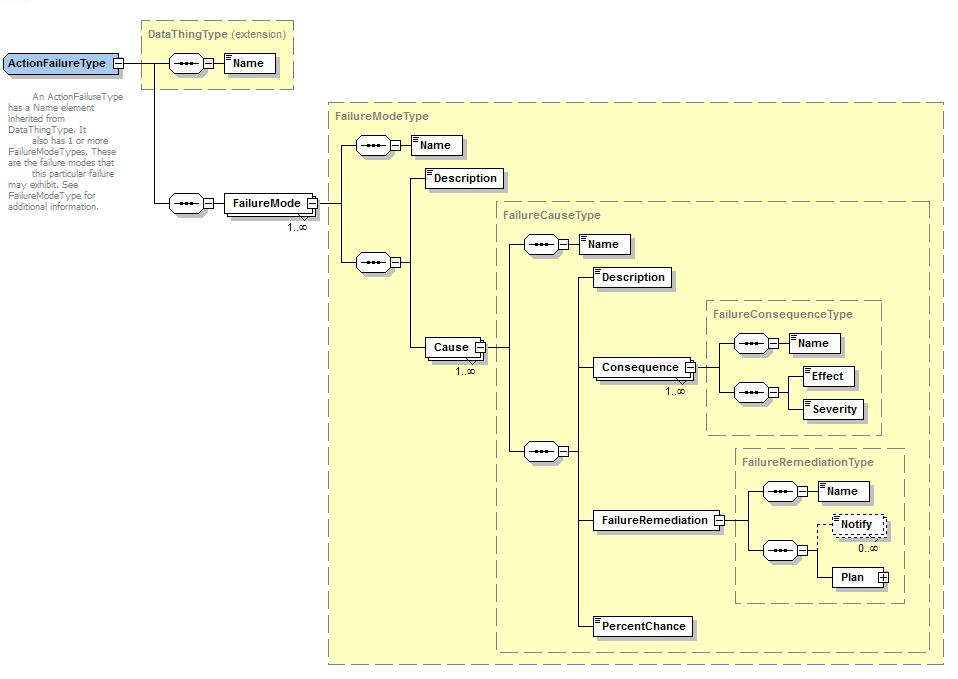
\includegraphics[width=12cm]{images/FailureType.jpg}
\caption{Description of the FailureType Class that is used to store information on action failures.}
\label{fig:failure}
\end{center}
\end{figure}
%
\section{Knowledge Representation}
\label{sect:knowledge}
%
\begin{algorithm}[h!]
\begin{tabbing}
\hspace*{.5cm}\=\hspace*{.5cm}\= \hspace*{.5cm}\= \kill
(:action place-part\\
\>	:parameters(\\
\>\>	?robot - Robot\\
\>\>	?stockkeepingunit - StockKeepingUnit\\
\>\>	?endeffector - EndEffector\\
\>\>	?kit - Kit)\\
\>	:precondition(and\\
\>\>	(endEffector-has-heldObject ?endeffector ?stockkeepingunit)\\
\>\>	(robot-has-endEffector ?robot ?endeffector)\\
\>\>	(equal-to (slot-found-flag) 1)\\
\>\>	(kit-has-slot ?kit))\\
\>	:effect(and\\
\>\>	(not(endEffector-has-heldObject ?endeffector))\\
\>\>	(set-value (slot-found-flag) 0)))\\
(:action look-for-slot\\
\>	:parameters(\\
\>\>	?robot - Robot\\
\>\>	?stockkeepingunit - StockKeepingUnit\\
\>\>	?kit - Kit)\\
\>	:precondition(and\\
\>\>	(equal-to (slot-found-flag) 1))\\
\>	:effect(and\\
\>\>	(set-value (slot-found-flag) 0)))\\
\end{tabbing}
\caption{Actions}
\label{fig:Actions}
\end{algorithm}
%
Two typical PDDL commands of {\it place-part} and {\it look-for-slot} 
are shown in Figure \ref{fig:Actions}. The {\it place-part} command
is used to put the currently held object into the ``slot'' of the kit
under construction that was found with the {\it look-for-slot} command.
If we assume that the action
{\it place-part} is being executed, then in line 4 of the {\sc BuildKit} algorithm
each of the predicates from the precondition section of the action 
will be verified. As previously mentioned, the evaluation of these predicates
could be hard-coded into the system. However, is there a more flexible way
that this could be accomplished?

\subsection{Predicate Representation}
If one examines each of the predicates that must be evaluated, it may be
noted that the predicates could be composed of a combination of simpler 
expressions. For example, the predicate expression:
\begin{gather} 
\class{endEffector-has-heldObject}(\textit{endeffector}, 
\textit{stockkeepingunit}),
\label{equation:endEffector-has-heldObject}
\end{gather}
is designed to verify that the robot's end-effector is holding the correct lass of part. It may be decomposed into the compound expression: 
\begin{gather}
\textbf{matchSKU}(\textbf{In-Contact-With}(\textit{endeffector}), stockkeepingunit)
\label{equation:matchSKU}
\end{gather}
In this case, \textit{endeffector} is the instance of the class end effector
that is expected to be attached to the robot
and 
\textit{stockkeepingunit} is the instance of the stock keeping unit
that belongs to the part that is expected to be held by the robot.
The expression \textbf{In-Contact-With} will determine what class of object is being held by the effector, while the expression \textbf{matchSKU} will determine if this represents the expected class.
 
The expressions \textbf{In-Contact-With} and \textbf{matchSKU}
are known as Intermediate State Relations (ISR) because the relate
complex elements of the system's state to easily measurable or
observable phenomenon. When called with a single parameter,
the measurable ISR of 
\textbf{In-Contact-With}(\textit{endeffector}) will return
a list of objects that are in contact with the end effector. 
This list will be passed as parameters to the observable
ISR of \textbf{matchSKU}. Since this relation is
expecting exactly two parameters, an end effector touching
zero or more than one object will result in an error. If a
single object is being held, it will be passed to \textbf{matchSKU} where
a simple observation may be made to see if the object's SKU
matches the one provided in the second parameter.

\subsubsection{RCC-8 Relation}
All of the measurable intermediate state relations may be further
decomposed into expressions that may be easily computed from
knowledge of the six degree-of-freedom pose of the objects. 
These base expressions are know
as Region Connected Calculus (RCC-8) relations and were originally
developed by Wolter and Zakharyaschev \cite{Wolter2000} 
as an approach for representing the relationship between two regions in 
Euclidean or topological space. 
RCC-8 consists of eight possible relations (hence RCC-8) that include
measurable region-to-region relationships such as
Tangential Proper Part (TPP) and Externally Connected (EC). 

In order to represent these relations in all three dimensions for 
industrial domains, RCC-8 has been extended to a three-dimensional space 
by applying it along all three planes (x-y, x-z, y-z) and by including 
cardinal direction relations ``+'' and ``-''. In our example of
Equation \ref{equation:matchSKU}, 
\textbf{In-Contact-With}(\textit{endeffector}) may be expressed
in RCC-8 relations as:
\begin{gather}
\textbf{In-Contact-With}(\textit{obj1}, \textit{obj2}) \rightarrow   \notag\\
\texttt{x-EC}(\textit{obj1}, \textit{obj2}) \vee \texttt{y-EC}(\textit{obj1}, \textit{obj2}) \vee \texttt{z-EC}(\textit{obj1},\textit{obj2}) \notag
\end{gather} 
Where \textit{EC} stands for Externally Connected, obj1 is the end effector, and obj2 is 
cycled through all of the detected objects in the work cell. 
\subsection{Observable Relations}
Work is still being performed to relate all of the simple observations to observable relations. In the case of the \textbf{matchSKU} observation, a \textit{model-match} or \textit{view-sku} operation could be performed. More on this topic is presented in Section \ref{sect:future}.
\subsection{Action Execution}
Once the precondition predicates have been validated, line 8 of the \textsc{BuildKit}
algorithm in Figure \ref{fig:buildkit} shows that the action should be executed. Once
again it is possible to decompose the complex actions into a much simpler form. 
In this case, two separate basis sets exist with one designed for the decomposition 
of Robot Actions and the other for the decomposition of Vision Actions.
%
\begin{figure}[htb!]
\begin{center}
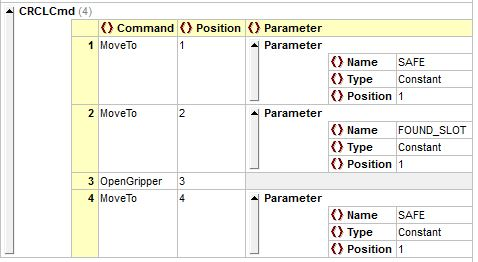
\includegraphics[width=8.5cm]{images/PlacePartCRCL.jpg}
\caption{The \textit{place-part} action may be decomposed into a sequence of
four CRCL commands.} 
\label{fig:PlacePartCRCL}
\end{center}
\end{figure}
%
\subsubsection{Canonical Robot Command Language}
The National Institute of Standards and Technology (NIST) has developed a
robot language known
as the Canonical Robotic Command Language (CRCL) that is designed to provide
a basis set of operations for robotic arms with industrial use 
cases \cite{Balakirsky2012-1}. This language contains 22 command elements that
may be sequenced to perform any of the PDDL Robot Actions that have been defined
for this domain. Continuing our example from above, 
Figure \ref{fig:PlacePartCRCL} displays the decomposition of the \textit{place-part} action.
As may be seen in the figure, the command decomposes into several movements and a gripper
command. The movements to a ``safe" location are not strictly necessary, but are
included to assure that the arm's motion begins and ends from a known safe position.
This position is a predefined constant in the system.
\textit{FOUND\_SLOT} is another system constant that represents a position buffer in 
the system. This buffer has previously been filled with the location of the actual
slot that is the destination of the part with the PDDL action 
\textit{look-for-slot}. 

Once the command execution is complete, the predicates that make up the effects
are examined in the same manner as the previously examined precondition predicates.
If any of the effects are deemed to have not occurred, then an error will be
generated.
\subsection{Instance Representation}
\label{sect:instance}
As discussed in the previous section, all of the PDDL predicates and actions may be
decomposed into a small set of primitives that includes
Robot Actions, Vision Actions, RCC-8 relations, and Observables. 
If this set of primitives is
programmed into the robot cell, then the set of behaviors that the cell is capable of
may be altered through the creation of new PDDL actions and predicates rather than
reprogramming the cell. In addition, these PDDL actions and predicates are independent
of the actual cell's implementation and product vendors. As long as the cell supports the
full set of primitives, it is capable of carrying out the operations without programming.

In order to translate PDDL predicates and actions into robot cell commands, 
the executor needs to have an
understanding of how the predicates and actions are composed. Since this information is
designed to not be hard-coded on the robot, it must be accessible to the running system.
In addition, since the actions and predicates are designed to be expanded upon as
new activities are added to the robot's vocabulary, the information needs to be
accessible in a human friendly form.
%
\begin{figure}[htb!]
\begin{center}
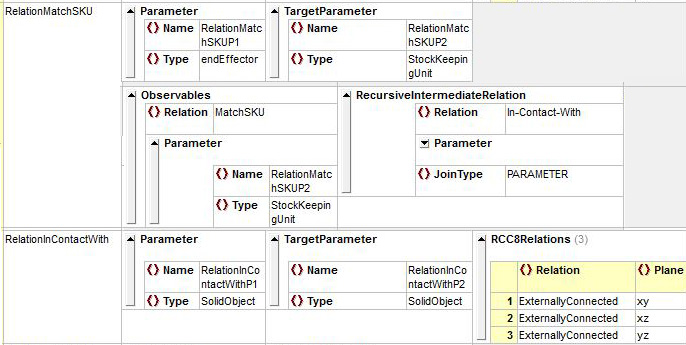
\includegraphics[width=12cm]{images/MatchSKU_ISR.jpg}
\caption{Intermediate State Relation RelationMatchSKU. This is the
implementation of Equation \ref{equation:matchSKU}.}
\label{fig:ISR}
\end{center}
\end{figure}
%
To meet all of these demands, this information is encoded in the Instance Ontology and is automatically entered into the Execution Model's MySQL database. 

The primitives themselves are implemented as simpleTypes in the schema.
In this case, the XML simpleType specifies an enumerated list of terms
that are within the robot and vision system's vocabulary. All of the
ISRs, predicates, and actions are composed of these elements, and these
elements are the only part of the system that is hard-coded onto the
robot.
\subsubsection{Intermediate State Relation}
The structure of the RelationMatchSKU ISR required by Equation \ref{equation:matchSKU} is shown in the XML
representation
depicted in Figure \ref{fig:ISR}. 
Recall from Equation \ref{equation:matchSKU} that this ISR is 
a recursive combination of the Robot ISR \textbf{In-Contact-With} and
the Vision ISR \textbf{MatchSKU}. This is shown in the XML in that
the \textit{RecursiveIntermediateRelation} is instantiated as
\textbf{In-Contact-With} with a single parameter of the end effector
and the \textit{JoinType} of \textit{PARAMETER}. This will cause a determination
of every object that is in contact with the effector. The 
determination of which objects are in contact with the effector
is made through the application of RCC-8 relations as shown in
the bottom part of Figure \ref{fig:ISR}. In this case, three
externally connected relations must be evaluated for each
object.The list of objects in contact
will get passed back as parameters to the \textit{MatchSKU} Vision ISR.
If zero or greater than one objects are passed to \textit{MatchSKU},
an error will be generated. If and only if one object is passed as
a parameter, that object's SKU will be compared against the target
SKU. Thus, from a combination of primitives we are able to determine
if the object being held by the end effector matches the SKU of the
expected object class. This in turn will deliver the truth value
of the predicate \textit{endEffector-has-heldObject()} depicted
in Equation \ref{equation:endEffector-has-heldObject}.  
\subsubsection{Actions}
\textit{CRCLActionTypes} and \textit{VisionActionTypes} are included
in the xml schema and are extensions of the \textit{ActionType} depicted
in Figure \ref{fig:ActionType}. These actions add the list of CRCL commands or observations that are required for the execution of the action. A sample of the CRCL commands for the \textit{place-part} action
are shown in Figure \ref{fig:PlacePartCRCL}. The encoding of all of the
actions is performed in the instance ontology.

\section{Conclusions and Future Work}
\label{sect:future}
The framework described in this paper has been applied to the domain of kit building, which is a simple, but practically useful manufacturing/assembly domain. Through its use, we have been able to demonstrate agility in both kit construction through late binding of part locations, and in recovery from action failures through the detection of failures and ability to compensate for the failure's effects.

There are several areas in the system that still utilize hand-coding of data. It is desired that extensions to the ontology be created that will allow for the automatic application of knowledge and eliminate code that it specifically tuned to a particular set of predicates or actions. The hand-coded areas include the conversion of PDDL actions to CRCL sequences as well as the retrieval of instance data from the MySQL database for predicate evaluation. Work is currently underway to correct for these deficiencies. 

Extensions are also possible that will expand this work to the realm of general assembly. We hope to apply this knowledge based framework to simple assembly tasks (growing towards more complex tasks) on a real robot workcell in the near future. 

%
%



%
% ---- Bibliography ----
%
%\bibliographystyle{plain}
\bibliography{ontology}
\end{document}
